\chapter{Tecnologias escolhidas}
\label{c.tecnologias}

% - Como cada um dos blocos propostos na seção anterior pode ser desenvolvido. Tecnologias podem ser microprocessadores, kits de desenvolvimento, linguagens de programação, protocolos de transmissão ou diferentes opções de algoritmos.
% - O aluno deverá fazer uma escolha inicial, justificada, da tecnologia que pretende utilizar.
% - As tecnologias escolhidas devem ser descritas com mais detalhes. As tecnologias concorrentes podem ser apresentadas de maneira resumida, mas com detalhe suficiente para caracterizar sua funcionalidade, bem como seus aspectos positivos e negativos.

Para implementar o projeto descrito, as seguintes tecnologias foram escolhidas:

\begin{itemize}
	\item Redis~\cite{redis}: banco de dados em memória de baixa latência. Utilizado para consultas eficientes por latitude e longitude e cache de tokens de sessão;
	\item PostgreSQL~\cite{postgresql}: banco relacional. Utilizado para persistência dos dados dos usuários, alertas e notificações;
	\item AWS~\cite{aws}: provedor de serviços em nuvem. Foi utilizado o serviço \emph{AWS S3} para armazenamento de objetos estáticos, como imagens e vídeos, e o serviço \emph{AWS RDS} para o provisionamento do banco de dados PostgreSQL;
	\item Heroku~\cite{heroku}: provedor de serviços em nuvem. Foi utilizado para o provisionamento do servidor e do Redis;
	\item Javascript~\cite{javascript}: linguagem de programação. Utilizada tanto no aplicativo quanto no servidor;
	\item Typescript~\cite{typescript}: sistema de tipos para Javascript. Utilizado tanto  no aplicativo quanto no servidor;
	\item GraphQL~\cite{graphql}: linguagem de consulta para APIs;
	\item Terraform~\cite{terraform}: ferramenta de \emph{Infrastructure as Code (IaC)} para gerenciamento serviços em nuvem via arquivos de configuração declarativos;
	\item Docker~\cite{docker}: ferramenta de virtualização à nível do sistema operacional. Utilizado durante o desenvolvimento isolado através de containers;
	\item Node.js~\cite{node}: \emph{Javascript runtime} construído sobre o motor V8 do Chrome. Utilizado para a escrita do backend (servidor);
	\item Koa~\cite{koa}: framework para contrução de servidor web no Node.js;
	\item Prisma~\cite{prisma}: \emph{Object-relational mapper (ORM)} para Node.js;
	\item Jest~\cite{jest}: framework para Node.js de testes unitários;
	\item Supertest~\cite{supertest}: framework para Node.js de testes de integração;
	\item React~\cite{react}: biblioteca Javascript para a construção de interfaces de usuário de forma declarativa;
	\item React Native~\cite{react-native}: framework híbrido para a construção de aplicações móveis que rodam em múltiplas plataformas (iOS e Android) utilizando React e Javascript. 	
	\item Expo~\cite{expo}: \emph{React Native runtime}, SDK e ferramenta para melhor experiência de desenvolvimento;
	\item Relay~\cite{relay}: framework e especificação para a busca de dados no React em servidores GraphQL, com foco em perfomance;
	\item Recoil~\cite{recoil}: biblioteca para gerenciamento de estado global no React;
	\item React Navigation~\cite{react-navigation}: biblioteca de navegação de telas no React Native.
\end{itemize}

A Figura~\ref{f.system} ilustra os componentes físicos do sistema e como eles se comunicam.

\begin{figure}[h]
	\caption{\small Componentes físicos do sistema.}
	\centering
	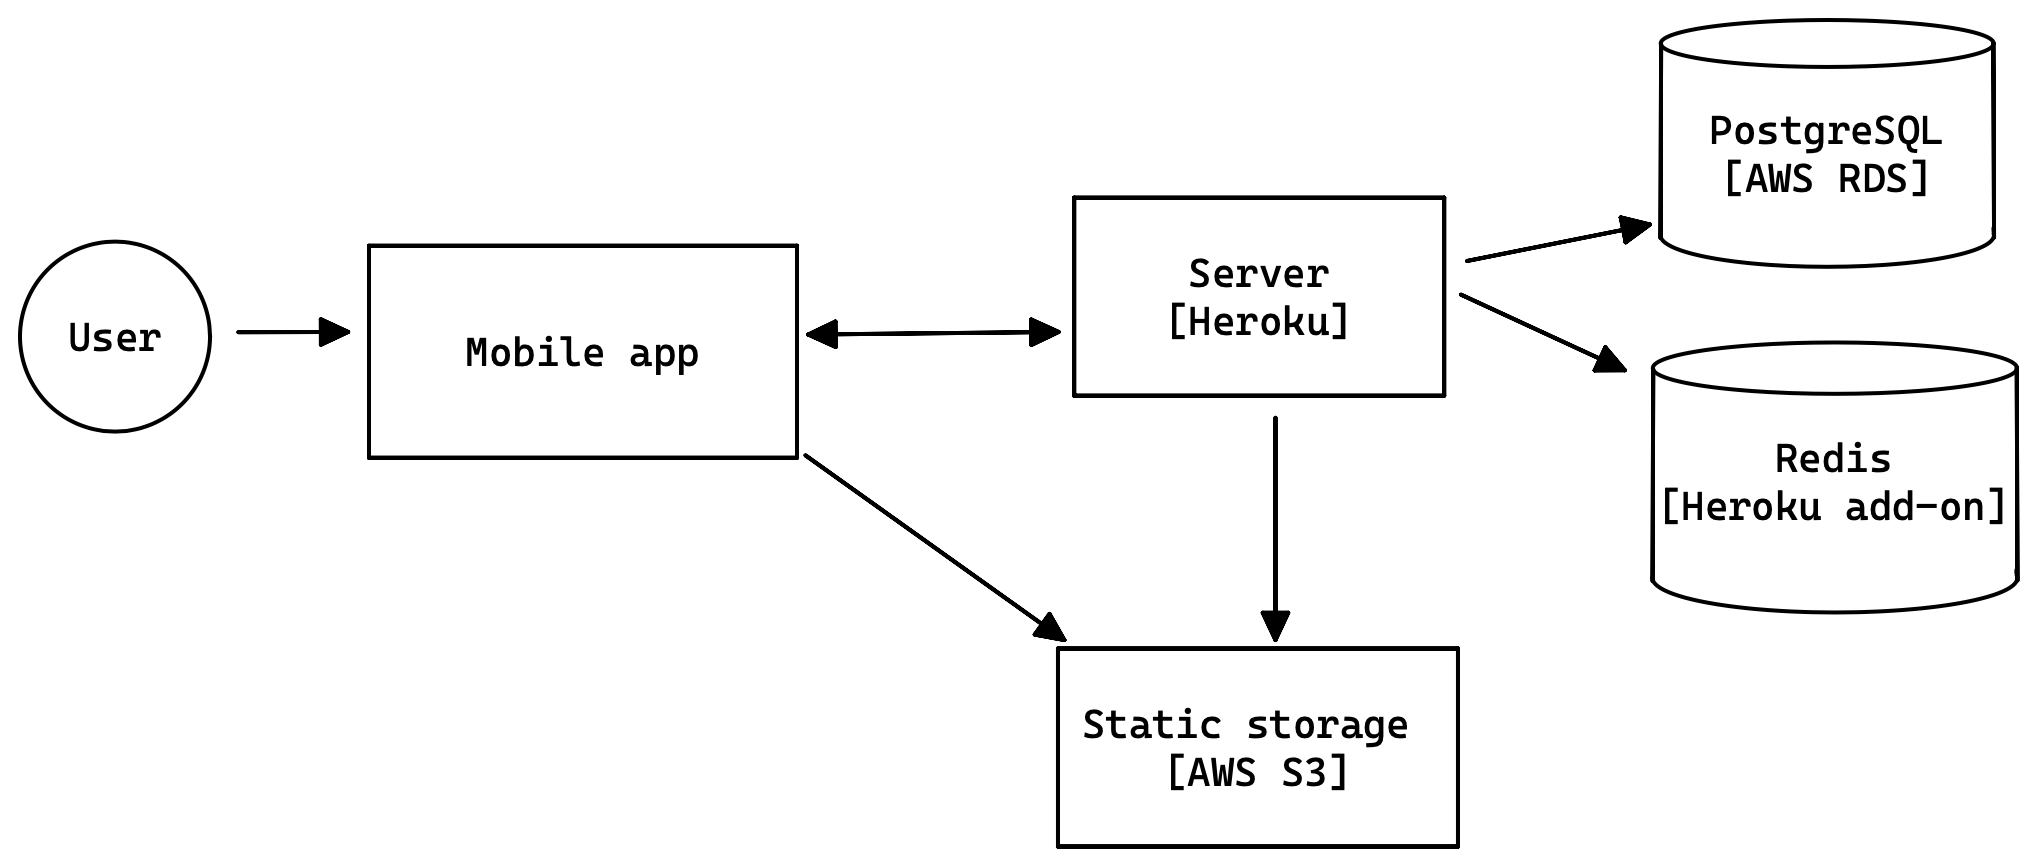
\includegraphics[width=\textwidth]{../diagrams/out/system.png}
	\label{f.system}
	\legend{\small Fonte: Elaborado pelo autor.}
\end{figure}

A Figura~\ref{f.system_server_api} ilustra de forma mais detalhada como o aplicativo se comunica com o servidor. Para \texttt{GraphQL queries} e \texttt{GraphQL mutations} há um fluxo síncrono de requisição-resposta e, portanto, é utilizado o protocolo HTTP, enquanto que para \texttt{GraphQL subscriptions} é estabelecida uma conexão persistente via o protocolo WebSocket, pois é uma comunicação assíncrona, ou seja, o servidor pode enviar atualizações ao cliente. No caso, alertas criados enquanto o usuário está com o aplicativo aberto, e próximos a ele, são enviados ao cliente, garantindo atualização de novos dados em tempo real ao aplicativo.

\begin{figure}[h]
	\caption{\small Interação detalhada entre cliente e servidor.}
	\centering
	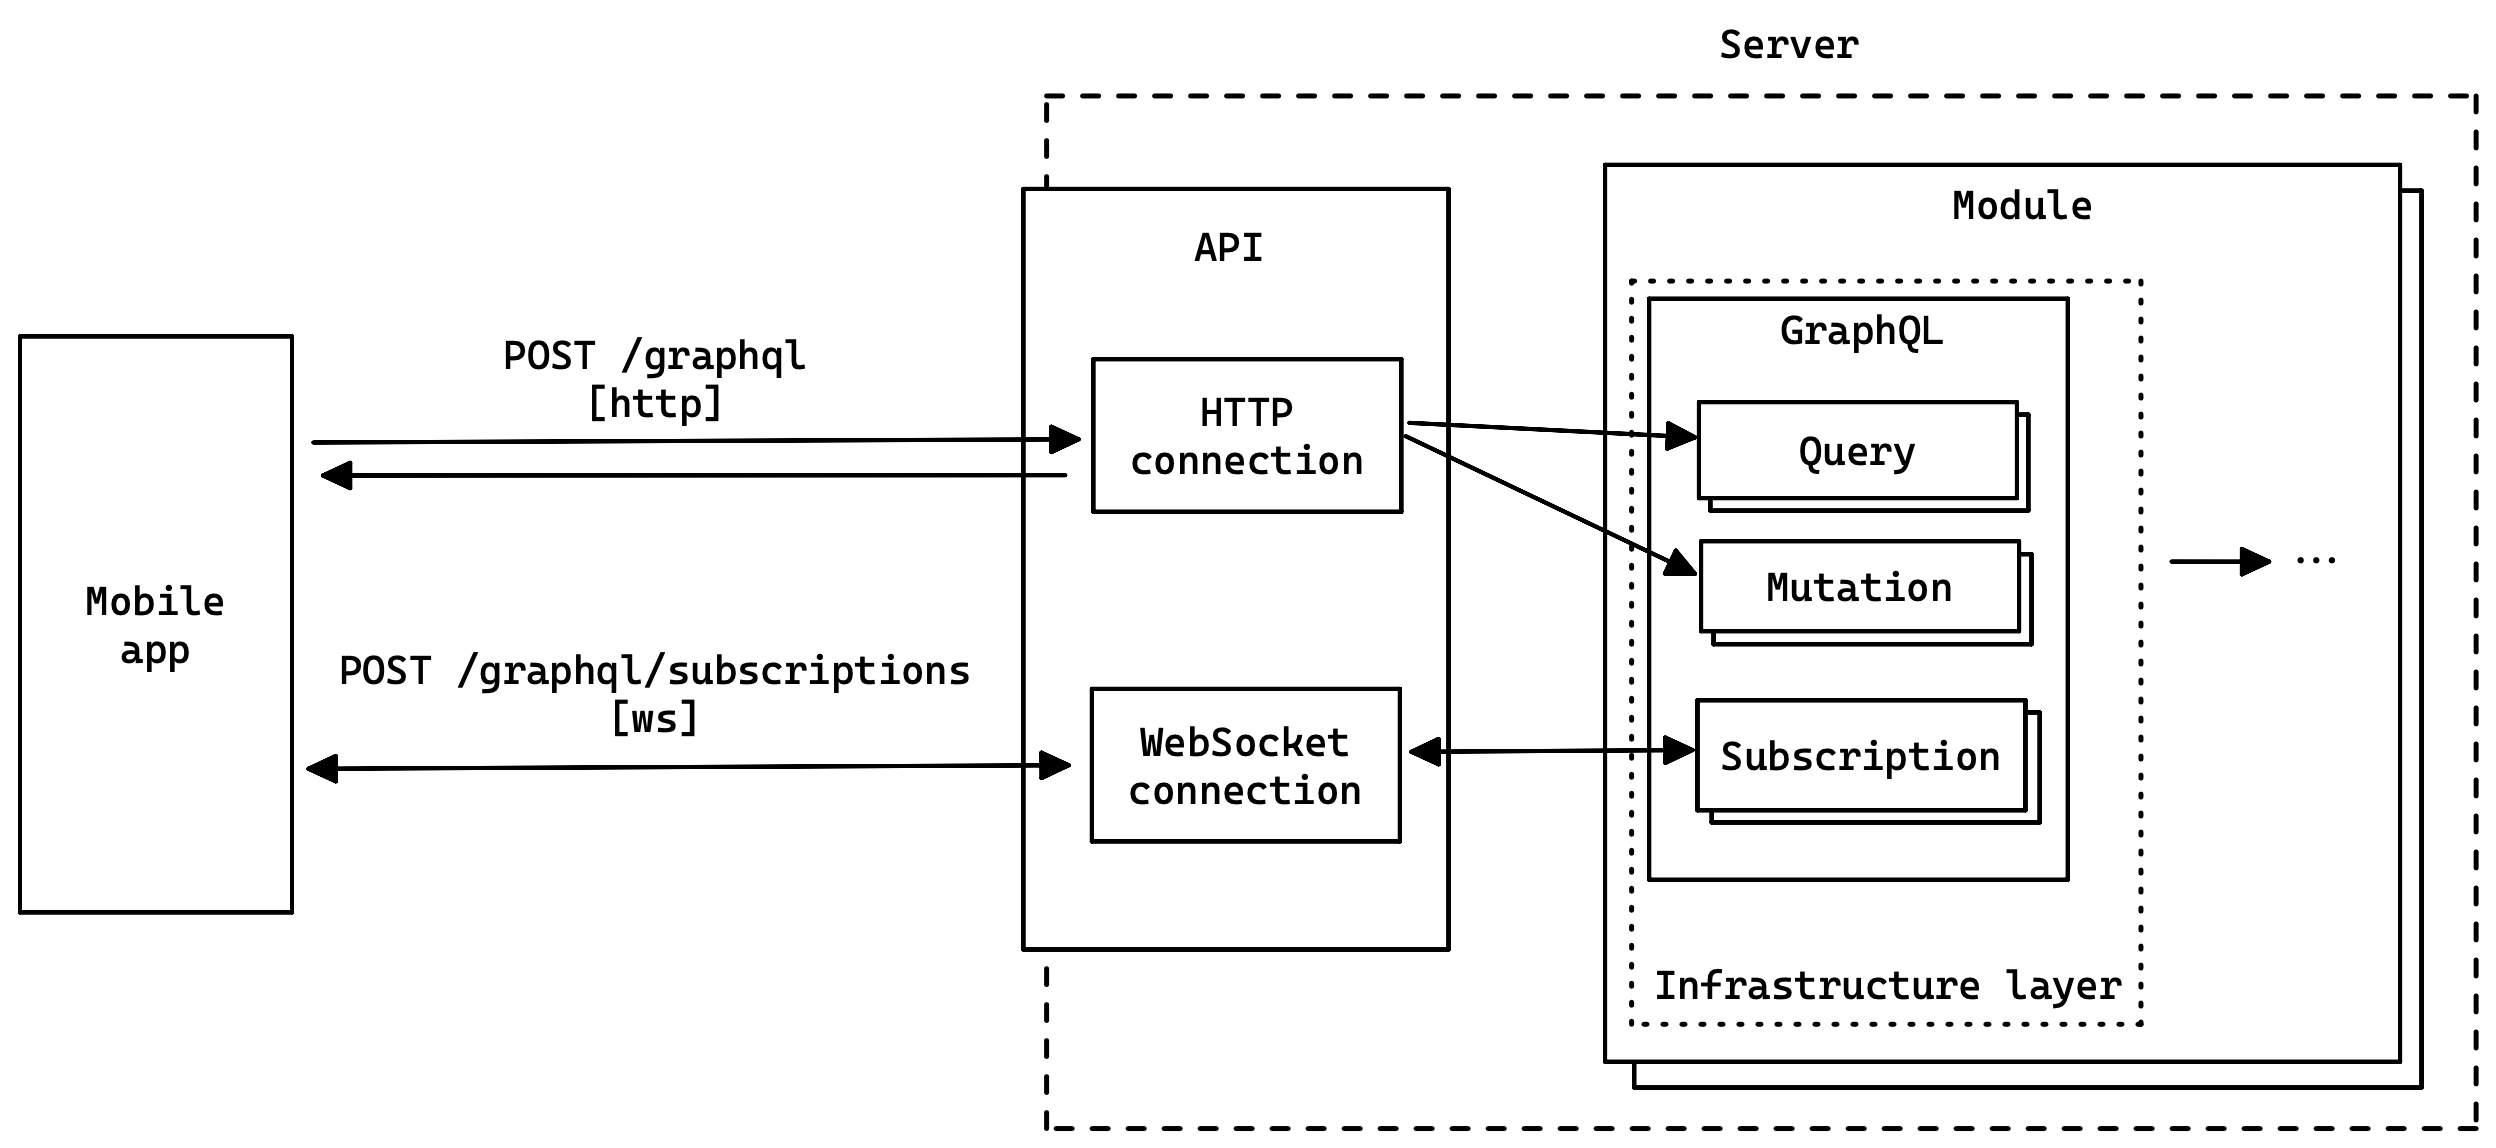
\includegraphics[width=\textwidth]{../diagrams/out/system_server_api.png}
	\label{f.system_server_api}
	\legend{\small Fonte: Elaborado pelo autor.}
\end{figure}

% \section{GraphQL ao invés de REST}

% \section{Servidor}
% \label{s.tecnologias-servidor}

% Escrito em Node.js


% \section{Aplicativo}
% \label{s.tecnologias-aplicativo}

% Escrito com React Native
% GraphQL
% Relay

% % TODO: diagram com: relay cache, graphql subscriptions, background location tracker, notifications listener, acesso ()


% \section{Desenvolvimento}

% Durante o desenvolvimento, as seguintes ferramentas foram utilizadas.

% Docker
% IaC - Terraform
% ORM - Prisma

% \section{Detalhes de implementação}
% % TODO: upload de imagens e vídeos

% Otimizando a consulta por incidentes localizados, dado um ponto central e um raio de distância

% utilizado a estrutura de dados \texttt{GEOSET};

% % Para atender o requisito de leituras com latência mínima, o banco de dados será modelado de forma otimizada para as leituras mais frequentes, como a consulta dos alertas próximos, dado uma localidade.

% % TODO: codigo do repositorio
% % TODO: incident & user data persisted view (redis <-> postgresql) pra mostrar como a query de incidents dentro de um raio é feita 

% % Para que o sistema proposto atenda o requisito não funcional de ser seguro, o cadastro de usuários deve ser único por número de celular ou e-mail, e oferecer opções de cadastro via provedores de identidade terceiros e autenticação em dois fatores.